\section{ETL}\label{sec:ETL}
The data foundation for this project relies on two sources, refer section \ref{sec:datafound}. Extract-Transform-Load(ETL) is an important phase for integrating these two sources of information into the data warehouse while ensuring a uniform data-representation. A preprocessing procedure fills static support-tables and dimensions with data. The data foundation contains data for car information and part of GPS Fact. After the preliminary data is loaded, a number of post-processing procedures fills the remaining tables in the data warehouse with data.

\begin{figure}[tb]
\centering
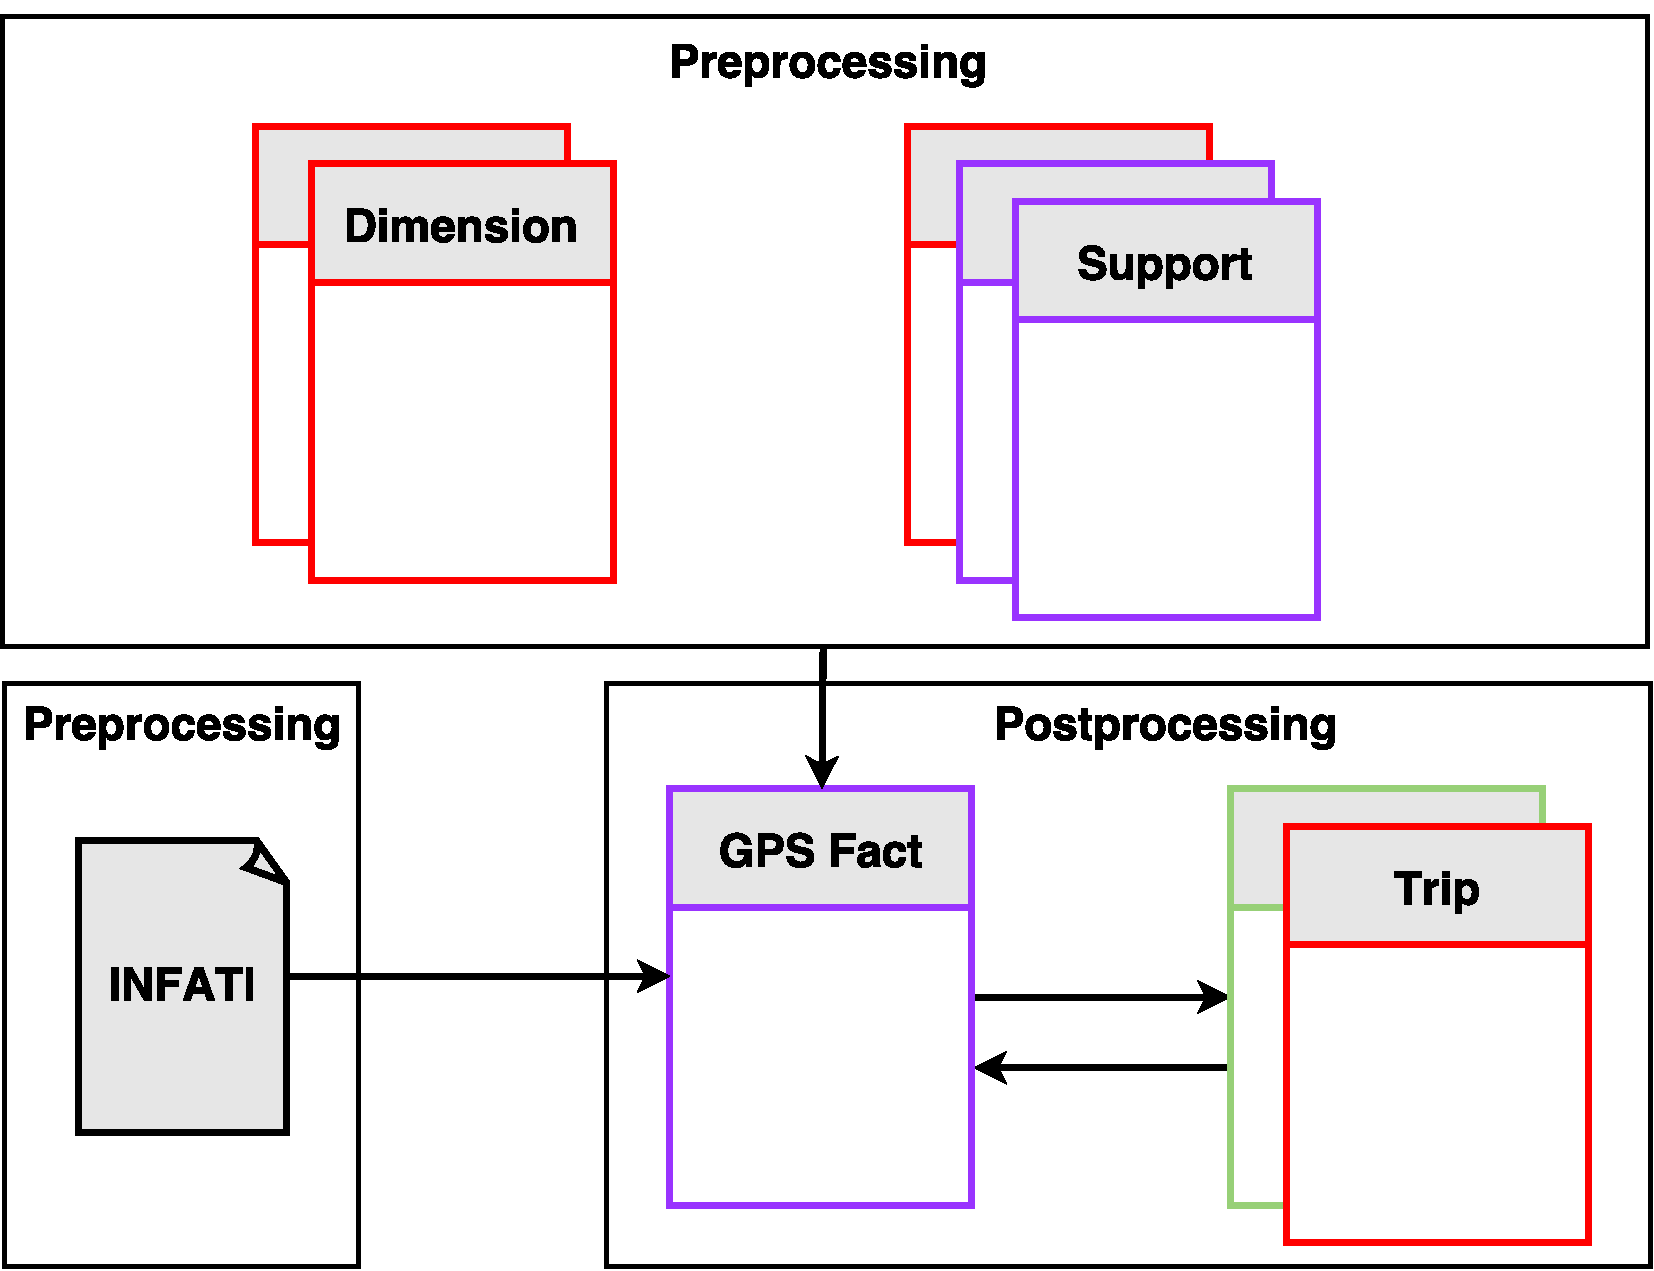
\includegraphics[width=0.465\textwidth]{Pictures/ETL}
\caption{Dataflow throughout the ETL process}
\label{fig:etl}
\end{figure}

The INFATI project\cite{art:INFATI} uses a digital roadmap from OpenStreetMap\cite{osm}. The same digital roadmap is used for this project. A few modifications is introduced, like storing the column \textit{direction} as a smallint instead of a textual representation. 

The INFATI dataset\cite{art:INFATI} contains 17 columns of data, separated by a varying number of spaces. Due to the natural challenges of map-matching, some entries contain only 14 columns of data. This causes the dataset to have problems with trailing zeros when loading with a space-separator. To ease the ETL process, a script has to be made for altering the separator. In this example \# is used, and whenever a row was not map-matched, three \#'s are appended to that row.

INFATI coordinate-sets are stored in Universal Transverse Mercator (UTM 32) format. This system is build on GPS, and a transformation from UTM to lattitude and longitude are needed. Coordinate-sets are stored as points, lines or polygons and stored in the data warehouse as PostGIS\cite{postgis} geometries. These geometries has to be assigned the correct spatial reference system identifier(SRID), otherwise they will refer to an incorrect positions. INFATI is logged in UTM32 North format, which has SRID 23032\cite{UTM32N}. Latitude and Longitude format is part of World Geodetic System(WGS), latest edition is WGS84 and has SRID 4326\cite{WGS84}. To transform the format: the geometry is created, assigned the UTM SRID, and transformed into WGS84 latitude longitude format using WGS84 SRID. 

Appropriate data for the support-table \textit{Quality Information} and the dimensions \textit{Date} and \textit{Time} are computed and stored. For \textit{Quality Information} this means storing each combination of HDOP and satellites.

The preprocessing is now complete, and the INFATI data can be loaded into the data warehouse. A car must be created and stored in \textit{Car Information}-table, hereafter the corresponding INFATI-data is loaded into the \textit{GPS Fact}-table. 

The postprocessing will now begin with dividing the batch of gpsfacts into trips for each car. Each found trip will be stored in the Trip Fact by a TripId and corresponding CarId, and the entire GPSFact-table will be updated for TripIds. 

\textit{GPS Fact} measures will then be calculated for all trips and cars. The process will take one car at a time, fetch all TripIds for that car, go over each trip and compute measures, update the gpsfacts with these measures.

When the \textit{GPS Fact} is updated with measures, it is possible to compute the measures for the Trip Fact-table. The process will take one car at a time, fetch all TripIds for that car, go by one trip at a time and fetch all gpsfacts for that trip. Whenever the measures have been calculated for a given trip, the Trip Fact is updated.

\textit{SubTrip Fact} is only conceptual at this time. It is not calculated and stored in the data warehouse. Though, it would primarily use the same computations as \textit{TripFact} which would make this process relatively trivial.

Given a working setting for the system, it could be another data-representation that the system would receive. This calls for designing and coding another ETL-procedure that can transform the data into the uniform data-representation present in the data warehouse.

%Måske skal det her ikke med?
To decrease the computation-time of the ETL-phase, the loading-process has been multi-threaded so that a single car is being loaded in its individual thread. This is only relevant for the INFATI dataset. In a working setting, data would come in bulks of single trips. 